\documentclass{layout/tudelft-aiaa}

%% Additional packages and commands
\renewcommand{\deg}{\si{\degree}\xspace}
\usepackage[newfloat]{minted} % (recommended)
\usepackage{comment}
\usepackage{biblatex}
\addbibresource{article.bib}
% Set global Minted options
\setminted{linenos, autogobble, frame=lines, framesep=2mm}

%% Defining title, author and affiliation
\title{A preCICE-OpenFAST adapter \\ to couple OpenFAST to CFD simulation tools \\ \vspace{4pt} \normalsize{Technical Report}}
\author{Leonard Willeke}
\affil{Delft University of Technology}

%%%%%%%%%%%%%%%%%%%%%%%%%%%%%
%%%%% Begin of document %%%%%
%%%%%%%%%%%%%%%%%%%%%%%%%%%%%

\begin{document}

\AlwaysPagewidth{

\maketitle

%% Abstract

\begin{abstract}
    \noindent
    Flow dynamics in wind parks are important for many engineering problems, ranging from optimized control to load reduction. This work introduces a preCICE-OpenFAST adapter designed to seamlessly couple OpenFAST with the preCICE library. preCICE facilitates the black-box coupling of simulation programs, enabling multi-physics simulations. The adapter acts as a driver code for OpenFAST, steering the turbine simulation and utilizing preCICE for efficient data exchange with the flow simulation. In a proof of concept, the adapter is employed to couple OpenFAST with OpenFOAM, demonstrating its potential despite limited capabilities. The presented approach lays the foundation for more comprehensive wind park simulations by integrating OpenFAST in the preCICE ecosystem. This research contributes to advancing wind park modeling techniques, providing a framework for studying complex interactions within wind farms.
\end{abstract}
}

%% Nomenclature

\renewcommand{\nompreamble}{\emph{Use this section to provide a list of all symbols used in the report. Provide a concise description. For example:}} %

\printnomenclature[\nomequalsign]

\nomenclature{$A$}{amplitude of oscillation}
\nomenclature{$C_p$}{pressure coefficient}
\nomenclature{$C_x$}{force coefficient in the x direction}
\nomenclature{$C_y$}{force coefficient in the y direction}
\nomenclature{$c$}{chord}
\nomenclature{$dt$}{time step}
\nomenclature{$F_x$}{X component of the resultant pressure force acting on the vehicle}
\nomenclature{$F_y$}{Y component of the resultant pressure force acting on the vehicle}
\nomenclature{$f, g$}{generic functions}
\nomenclature{$h$}{height}
\nomenclature{$i$}{time index during navigation}

%% Main body

\section{Introduction}

\lettrine{T}{his} template is a simple article template following all the guidelines of AE2333-I, based on the official AIAA template. Refer to the AE2333-I Word template to see all the procedures and guidelines. Please note that you are free to use other formatting styles, as long as you are consistent in how you apply them throughout your text. By default, the article is in one column. Switching to two columns can be done using the \emph{twocolumn} global option, resulting in the following first line in article.tex: \emph{\textbackslash documentclass[twocolumn]\{layout/tudelft-aiaa\}}.


\section{Literature Review}
\label{section:review}

A recent advancement in the coupling of OpenFAST is the tool \textbf{AspFAST} \cite{Taschner:2022}. Developed at the Delf University of Technology and the weather forecasting company Whiffle, it connects OpenFAST to the closed-license Large Eddy Simulation (LES) code GRASP. 
As a binder code, AspFAST serves as an intermediary between the GPU-driven GRASP and the CPU-driven OpenFAST. It accesses OpenFAST through a C++ API, essentially operating as a driver code. GRASP is accessed through a specialized API that handles the transition from CPU to GPU operations.
The core functionalities of AspFAST include the data exchange and mapping between GRASP and OpenFAST. This is done for crucial data such as force, velocity, and the position of turbine blades. Notably, the code implements the mapping between the volume-based velocity grid of GRASP and the actuator line model of OpenFAST. Because the coupling  code\footnote{\url{https://gitlab.com/whiffle-public/aspfast} (visited on 20.12.2023)} is open-source, it can serve as a blueprint for anyone interested in coupling OpenFAST via the C++ interface.
The software architecture of AspFAST is not far from our idea for the preCICE-OpenFAST adapter: AspFAST is a plug-in for the CFD solver GRASP while being the driver code for OpenFAST, serving as the "adapter" between the two. A big difference lies in the fact that AspFAST also has to implement the mapping algorithms, which are executed by preCICE in our approach.

The \textbf{ExaWind} project \cite{Sprague:2019} is based on the open-source, massively paralles and incompressible flow solver NaluWind \cite{Ananthan:2019}. It is a wind-focused adaption of the general flow solver NaluCFD and strives to deliver flow simulations in exascale. Hence, great emphasis lies on the scalability and simulation speed of the software through advanced solver and coupling algorihtms as well as the use of GPUs. The coupling to OpenFAST is implemented inside NaluWind and not as additional plug-in. An extensive documentation with insights into the theory and verification is given. 

Another coupling based on solver modification is the Simulator for Wind Farm Applications or \textbf{SOWFA} \cite{Churchfield:2012} from NREL. It couples OpenFOAM to OpenFAST by providing an additional  class \textit{horizontalAxisALM} in OpenFOAM. It defines functions to call OpenFAST and enables the data exchange. This class can be included directly in any OpenFOAM solver by modifying the OpenFOAM source code, so that the solver calls OpenFAST during each time step.

A software solution relying on a similar coupling tool to preCICE is \textbf{foamFAST} \cite{Weber:2017}. This project uses the commercial coupling tool for partitioned multi-physics simulations MpCCI, developed and sold by the Fraunhofer SCAI. Similar to preCICE, MpCCI is connected to different programs via adapters. Once the adapter is written, you can couple your tool to any other tool in the MpCCI environment. A difference in software architecture is the fact that MpCCI acts as the master algorithm: It calls the solvers instead of being called by them like preCICE. During the project, a MpCCI adapter for OpenFAST was developed and an existing OpenFOAM adapter modified to perform the coupling between the two.\\

The reviewed literature shows two different concepts to undertake the coupling. The first idea is to \textbf{modify the CFD solver source code}, as the ExaWind project has done with the NaluWind solver and SOWFA with OpenFOAM. While convenient for developers who are familiar with the software, this approach can prove hard to maintain when the underlying solver software is updated.

The second concept leaves the CFD solvers intact and uses \textbf{an additional software layer} to connect the simulation tools. One way to implement this is the library approach where an additional module or library is called by the original CFD solver. An example is AspFAST, where the stand-alone plug-in code is maintained seperately from the solver. The second way for implementation is the framework approach, used by the coupling tool MpCCI in foamFAST. Here, the additional software acts as a master algorithm calling the solver.

Given the previous work, why should we continue to develop a preCICE-OpenFAST adapter?
Our approach combines some of the positive aspects of previous projects. First, preCICE follows the library approach, leaving the original programs untouched and enabling a fast time-to-solution. Using preCICE allows to rely on advanced and tested coupling algorithms without the need to re-implement them or buy a licensed software. Establishing a preCICE-OpenFAST adapter opens up the road to connect OpenFAST not only to OpenFOAM, but to any CFD solver coupled to preCICE. Furthermore, preCICE creates a clean and easy to use simulation environment and simplifies setting up and maintaining simulations.

Nevertheless, it should be noted that OpenFOAM is currently the only CFD solver connected to preCICE which can be used for a coupling with OpenFAST. Coupling any other tool, such as the presented GRASP or NaluCFD, will require the development of additional adapters.

\begin{comment}
% Not relevant for our case
\textbf{OF2: A coupling library for OpenFOAM}
\begin{itemize}
\item Motivation: Model FOWTs with mixed fidelity to speed up the design process
\item OpenFOAM computes the floater hydrodynamics with high fidelity
\item OpenFAST computes the rotor aerodynamics and servo-elastic response in low-fidelity
\item Method: Two OpenFOAM libraries perform the coupling
\item libForcedOpenFAST: Software layer to interact with and execute OpenFAST
\item libOF2: Software layer to read and write data from OpenFOAM
\item Both libraries communicate with each other
\item Benefits: Less computationally expensive than CFD only, simulation of large turbine displacements (drift, rotation) possible
\item Drawbacks: Done for hydrodynamics (OpenFOAM replaces HydroDyn), not sure if this approach would work for aerodynamics as well (yes)
\\
\end{itemize}

% Used
\textbf{AspFAST} \cite{Taschner:2022}
\begin{itemize}
\item Motivation
\begin{itemize}
\item Wind farm simulation combines the analysis of large-scale flow dynamics with individual turbine behavior
\item Different tools are needed to model these two phenomena
\item AspFAST couples the LES code GRASP with the wind turbine tool OpenFAST to perform such simulations
\end{itemize}
\item Methodology
\begin{itemize}
\item AspFAST is a binder code between the GPU-driven GRASP and the CPU-driven OpenFAST
\item OpenFAST is accessed via C++ API → AspFAST is the driver code
\item AspFAST takes care of the mapping and communication between the tools
\end{itemize}
\item What AspFAST does
\begin{itemize}
\item Synchronize GRASP and OpenFAST
\item Exchange data: Force, Velocity, Position (of the turbine blades)
\item Map data and make use of the actuator line model
\begin{itemize}
\item Map velocity from GRASP to OpenFAST
\item Map force from OpenFAST to GRASP
\item Make use of both internal meshes inside of OpenFAST
\end{itemize}
\end{itemize}
\item How it relates to our idea
\begin{itemize}
\item Very close to what we want to achieve
\item Difference: GRASP is a commercial and licensed software, AspFAST allows coupling only to this one solver
\item But: AspFAST itself is open-source and can serve as a blueprint
\item The coupling of the parallel flow solver NaluWind with OpenFAST pursues a very similar idea
\\
\end{itemize}
\end{itemize}

\textbf{ExaWind: A Coupling of NaluWind with OpenFAST} \cite{Sprague:2019}\\
\begin{itemize}
\item NaluWind is an open-source massively parallel, incompressible flow solver for wind turbines and parks
\item Is a wind-focused adaption of the general flow solver NaluCFD
\item Focus on delivering flow simulations in exascale
\item Coupled to OpenFAST to perform multi-fidelity simulations of wind parks
\item Verified simulation on single turbine case against other codes and experiments
\item Emphasis on scalability and increased simulation speed through advanced solver and coupling algorithms and the optional use of GPUs
\item Extensive documentation with insights into the theory and verification 
\item How does it relate to our work
\begin{itemize}
\item Very close to what we want to do
\item Especially interesting for high-performance applications
\item Expert tool that needs some time to set up, understand, and run --> The hope is that our coupling to the "standard" tool OpenFOAM will have a lower barrier for beginners
\end{itemize}
\end{itemize}

\textbf{SOWFA} \cite{Churchfield:2012}
\begin{itemize}
\item Developed by NREL
\item Simulator for Wind Farm Applications based on OpenFOAM
\item Enables a coupling with OpenFAST
\item Methodology
\begin{itemize}
\item Implements a turbine class horizontalAxisALM in OpenFOAM to call OpenFAST and exchange data
\item This class can be included in any OpenFOAM solver
\item The solver calls OpenFAST during each timestep
\end{itemize}
\item How this relates to our idea
\begin{itemize}
\item Different approach: Is based on the modification of OpenFOAM source code while we strive to leave the solvers untouched
\item A lot of internal OpenFOAM knowledge necessary
\\
\end{itemize}
\end{itemize}

\textbf{foamFAST and MPCCI coupling tool} \cite{Weber:2017}
\begin{itemize}
\item Motivation
\begin{itemize}
\item Replace the low-fidelity aerodynamic calculations in FAST, based on the BEM theory, with high-fidelity calculations in OpenFOAM
\item BEM theory is not sufficient for many applications; CFD is needed
\item Use the coupling tool MpCCI to perform the coupling
\end{itemize}
\item Methodology
\begin{itemize}
\item Couple OpenFOAM and OpenFAST via the coupling tool MpCCI
\item MpCCI is a licensed coupling tool for partitioned multi-physics simulations developed by the Fraunhofer SCAI
\begin{itemize}
\item Connect tools to MpCCI via adapters
\item Once the adapter is written, you can couple your tool to any other tool connected to MpCCI
\item MpCCI acts as the master algorithm
\end{itemize}
\item This project developed an OpenFAST adapter from scratch and adapted an existing OpenFOAM adapter to perform the coupling
\item Source code is not violated
\end{itemize}
\item How it relates to our idea
\begin{itemize}
\item Very similar approach to preCICE´
\item Difference of MpCCI and preCICE: preCICE takes the library approach, while MpCCI takes the master algorithm approach
\item MpCCI is commercial and has limited HPC capabilities
\\
\end{itemize}
\end{itemize}

\begin{itemize}
\item Combines positive aspects of previous works while avoiding some drawbacks
\item Maintainability: Adapter is a separated piece of code which is easier to maintain than a modified OpenFOAM solver
\item Open access: No license
\item Plug and play: Adapter opens the road to connect OpenFAST not only to OpenFOAM, but to any CFD solver coupled to preCICE
\item Easy to use: preCICE creates a clean simulation environment, seperating the coupled tools clearly, from which students and professionals benefit
\end{itemize}
What are some serious drawbacks?
\begin{itemize}
\item There are currently no preCICE adapters for other CFD solvers that would be interesting to couple to: NaluWind, GRASP, ...
\item Developing such adapters would mean to re-implement a functionality that already exists in native coupling tools --> questionable if that is a good investment
\end{itemize}

\end{comment}

\section{Software description}

\subsection{Software components}

\subsubsection{preCICE}
\begin{itemize}
	\item An overview is shown in Figure \ref{fig:precice:overview}
	\item Coupled simulation programs are called \textit{solvers} or \textit{participants}
	\item preCICE connects different solvers to perform a partitioned simulation
	\item preCICE takes care of different coupling aspects such as data mapping and communication
	\item Different coupling schemes can be implemented: Who is coupled o whom, what data is exchanged, which coupling algorithms are used \cite{Gatzhammer:2014}
	\item Multi-coupling: Couple multiple (in theory: arbitrary many) participants in different configurations (explicit, implicit)
	\item Acceleration: Use acceleration algorithms to reach a decent computation time
	\item Time interpolation: Use solvers with different time step sizes
	\item Coupling scheme is defined in the precice-config.xml, the only global file which is accessed by all participants
	\item For each solver, a specific \textit{adapter} is necessary to communicate to preCICE
	\item Adapter is an additional piece of software
	\item Adapter can take many forms depending on the solver, eg.: OpenFOAM - C++ Function object, FEniCS - Python module
	\item Different Language bindings are available: C/C++, Python, Fortran, Julia, Matlab
	\item The Adapter allows the solver to access preCICE and to call the coupling
\end{itemize}

\begin{figure*}[t]
	\centering
	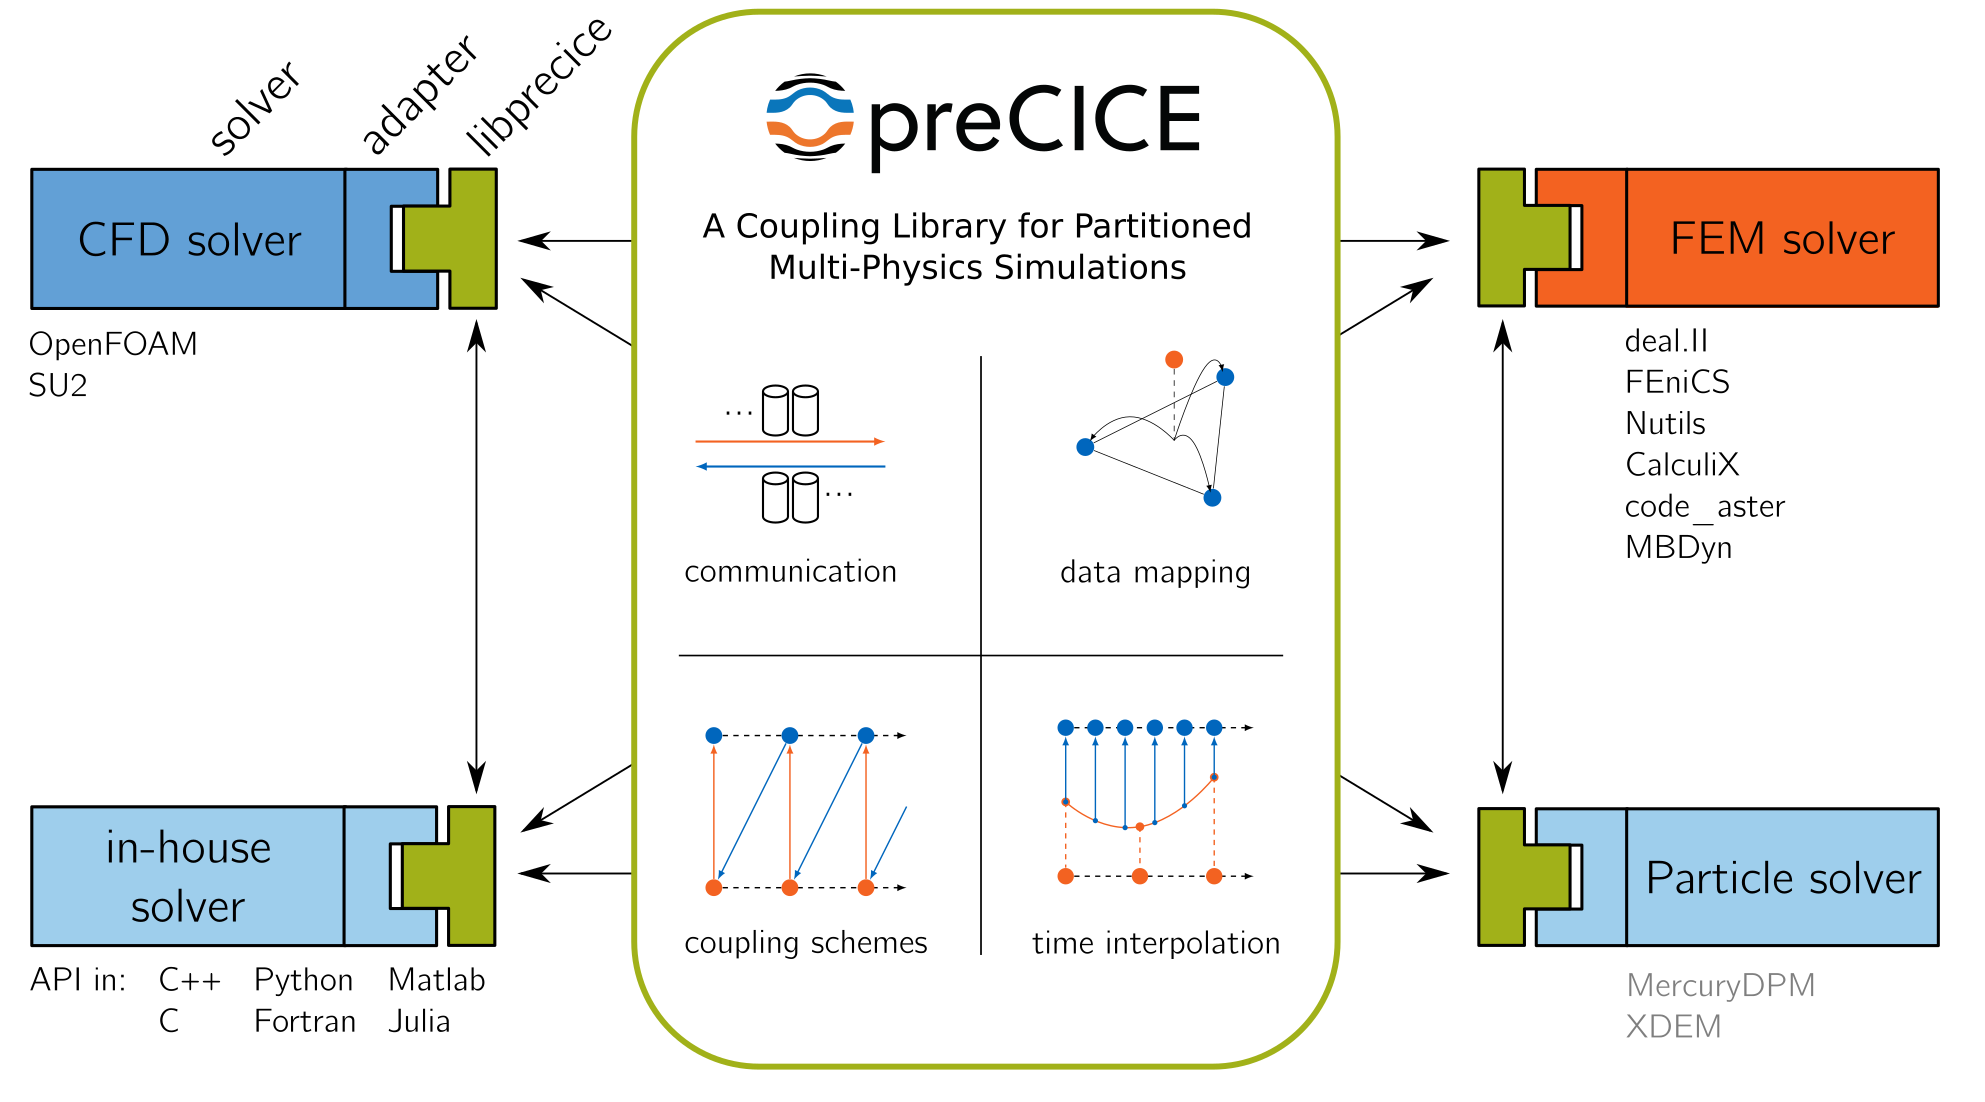
\includegraphics[width=0.9 \textwidth]{images/precice-overview.png}
	\caption{preCICE overview \cite{Chourdakis:2022}}
	\label{fig:precice:overview}
\end{figure*}


\subsubsection{OpenFOAM and the preCICE-OpenFOAM adapter}
\begin{itemize}
	\item OpenFOAM
	\begin{itemize}
		\item Popular open-source PDE tool in academia and industry
		\item Enables the use and modification of different solvers
		\item Used mainly for CFD but also FEM simulations 
	\end{itemize}
	\item Adapter
	\begin{itemize}
		\item Enables the coupling of OpenFOAM via preCICE in different simulation scenarios
		\item Exemplifies the development strategy behind preCICE: Adapter is a library for OpenFOAM and called on runtime to perform the coupling without any modification to the OpenFOAM source code
		\item Different modules for different kinds of multi-physics simulations: FSI, FF, CHT
	\end{itemize}
\end{itemize}	
Note:
I should introduce the OpenFOAM adapter at some point.
Lets introduce the broad concept of the adapter here and add more details, eg about the specific files that would need to be modified, later in the Challenges part
\newline
\subsubsection{OpenFAST}
\begin{itemize}
	\item Wind energy engineering tool developed by NREL
	\item Widely used in academia and industry
	\item Simulates the coupled aerodynamic, structural, and electrical behaviour of wind turbines as well as the control response
	\item Allows to model on- and offshore wind turbines and can be used to compute wind parks as well
	\item OpenFAST is a glue code for different modules which compute the various physical domains
	\item Takes one main input file denoted \textit{.fst} which points to more specific files for each computation module (eg AeroDyn, ServoDyn, ...)
	\item Fidelity: Does OpenFAST include computations in different fidelities? Is it a low- to mid-fidelity tool?
	\item Computes the Fluid-Structure-Interaction at blades and tower with the actuator line method
	\item Inflow field is either computed by AeroDyn or received from external CFD solver
	\item Has a dedicated C++ API for the coupling with CFD solvers
\end{itemize}

OpenFAST is mainly used to perform turbine loads analysis and drive the detailed turbine design. The computational cost is therefore higher than for tools used in the early design exploration phase like WISDEM, RAFT or FLORIS, but lower than highly resolved solvers necessary to understand the actual physics and check the final turbine design like ExaWind or SOWFA. 

\subsection{Software concept}

Main idea
\begin{itemize}
	\item Write a preCICE-OpenFAST adapter (see Figure \ref{fig:setup}), a new piece of software that connects OpenFAST and preCICE
	\item Acts as driver code towards OpenFAST: Calls it via the C++ API
	\item Calls preCICE to communicate data and steering commands
	\item Configurable by two .yaml input files
	\item preciceSettings.yaml contains information about the coupling setup
	\item openfastSettings.yaml contains information about the turbine simulation case
	\item The concept is sketched out in Figure \ref{code:adapter}
	\item line 8-10: Instantiate and initialize the interface to OpenFAST
	\item line 12-14: Do the same for preCICE
	\item Now both software component are ready to use
	\item line 16: main time loop controlled by preCICE
	\item line 18: Read velocity data from CFD solver via preCICE and store it in local variable
	\item line 20: Set the velocity data in OpenFAST
	\item line 22: Tell OpenFAST to compute the wind turbine dynamics for the next time step
	\item line 24: Get the resulting force from OpenFAST and store it in local variable
	\item line 26: Send force data to CFD solver to be used in ALM method
	\item line 28: Advance both solvers in time
	\item line 30-31: End the simulation after the main loop has finished
	\item Developed and documented on GitHub\footnote{\url{https://github.com/LeonardWilleke/openfast-adapter}}\\
\end{itemize}

\begin{comment}
	The OpenFAST adapter is something between the FMI Runner and a normal adapter:
	It executes OpenFAST like the runner but OpenFAST is a full, executable program on
	its own.
	
	\begin{figure*}[t]
	\centering
	\includegraphics[width=0.9 \textwidth]{images/precice-openfast-adapter-setup.png}
	\caption{preCICE-OpenFAST Adapter software architecture}
	\label{fig:openfast:adapter}
	\end{figure*}
\end{comment}


\begin{figure}[h!]
	\centering
	\begin{minipage}{0.9\textwidth}
		\begin{minted}{cpp}
		#include <OpenFAST.H>
		#include <precice.hpp>
		
		vector<double> readData;
		vector<double> writeData;
		
		// OpenFAST Setup
		fast::OpenFAST FAST;
		...
		FAST.init()
		// preCICE Setup
		participant = precice.participant(...);
		...
		participant.initialize();
		// main time loop
		while participant.isCouplingOngoing(): 
			// Get read data from preCICE
			participant.readData(readData, ...);
			// Set read data in OpenFAST
			FAST.setVelocity(readData, ...);
			// Compute next time step
			FAST.step();
			// Get write data from OpenFAST
			FAST.getForce(writeData, ...);
			// Send write data to preCICE
			participant.writeData(writeData, ...);
			// Advance preCICE in time
			participant.advance(dt) 
		
		participant.finalize()
		FAST.end()
		\end{minted}
	\end{minipage}
	\caption{Concept of the OpenFAST adapter: The script utilizes the C++ API to execute OpenFAST and calls preCICE to couple the simulation. For conciseness, API calls are simplified.}
	\label{code:adapter}
\end{figure}


\section{Example cases}
\label{section:cases}

To drive the adapter development and test the software at its current state, two example cases were implemented. The OpenFAST simulation of a single wind turbine, namely the NREL 5MW model \cite{Jonkman:2009}, is coupled. The first case implements the coupling to a dummy fluid solver. While performing no realistic computations, the dummy is handy to get an insight into the different data structures, mesh setups, and mapping options. The second case couples OpenFAST to the CFD program OpenFOAM. It can be seen as a first proof-of-principle with a successful data exchange via preCICE. However, more work needs to be done to ensure a correct and robust simulation. Both cases are part of the repository on GitHub\footnote{\url{https://github.com/LeonardWilleke/openfast-adapter/tree/main/cases}}.

\begin{comment}
\begin{itemize}
\item Two example cases were implemented to drive the adapter development
\item The OpenFAST simulation of a single NREL 5MW turbine \cite{Jonkman:2009} should be coupled
\item Coupling to dummy fluid solver to test the data exchange
\item Coupling to OpenFOAM to test the mapping with a CFD tool
\item Both cases are part of the repository on GitHub\footnote{\url{https://github.com/LeonardWilleke/openfast-adapter/tree/main/cases}}\\
\end{itemize}
\end{comment}

\subsection{Coupling OpenFAST with a dummy CFD solver}

The motivation for this case is to provide a simple and fast way to test different functionalities and gain insight, not to perform realistic simulations. OpenFAST computes a NREL 5MW turbine with a fixed rotor to avoid mesh problems on the moving blades. The fluid solver is implemented as a simple C++ script. It creates a mesh that can be used to map data from OpenFAST and write constant values back. The dummy does not perform any calculations. To perform the coupling, the script calls preCICE. This case allows to explore the mapping and data exchange in a minimal setup.

OpenFAST employs two internal meshes of the turbine surface with different vertices. Force data is stored on one mesh, while flow velocity is stored on another. Both meshes can be accessed by the C++ API. However, it is also possible to exchange both variables on the velocity mesh only and call an internal mapping function in OpenFAST to map the force data to the force mesh. Inspired by the coupling setup in \cite{Taschner:2022}, I want to access both meshes and use preCICE for the mapping. This results in the elaborous coupling scheme seen in Figure \ref{fig:openfast:coupling}. In total, three meshes are employed: The Fluid solver has one mesh \textit{Fluid-Mesh} used for both the force and velocity data while the Solid solver (OpenFAST) uses two meshes. \textit{Solid-Mesh-Velocity} is the velocity mesh of OpenFAST, on which the velocity data from the Fluid solver is mapped. \textit{Solid-Mesh-Force} is the force mesh of OpenFAST, from which force data is mapped back to the Fluid solver.

\begin{figure*}[h]
	\centering
	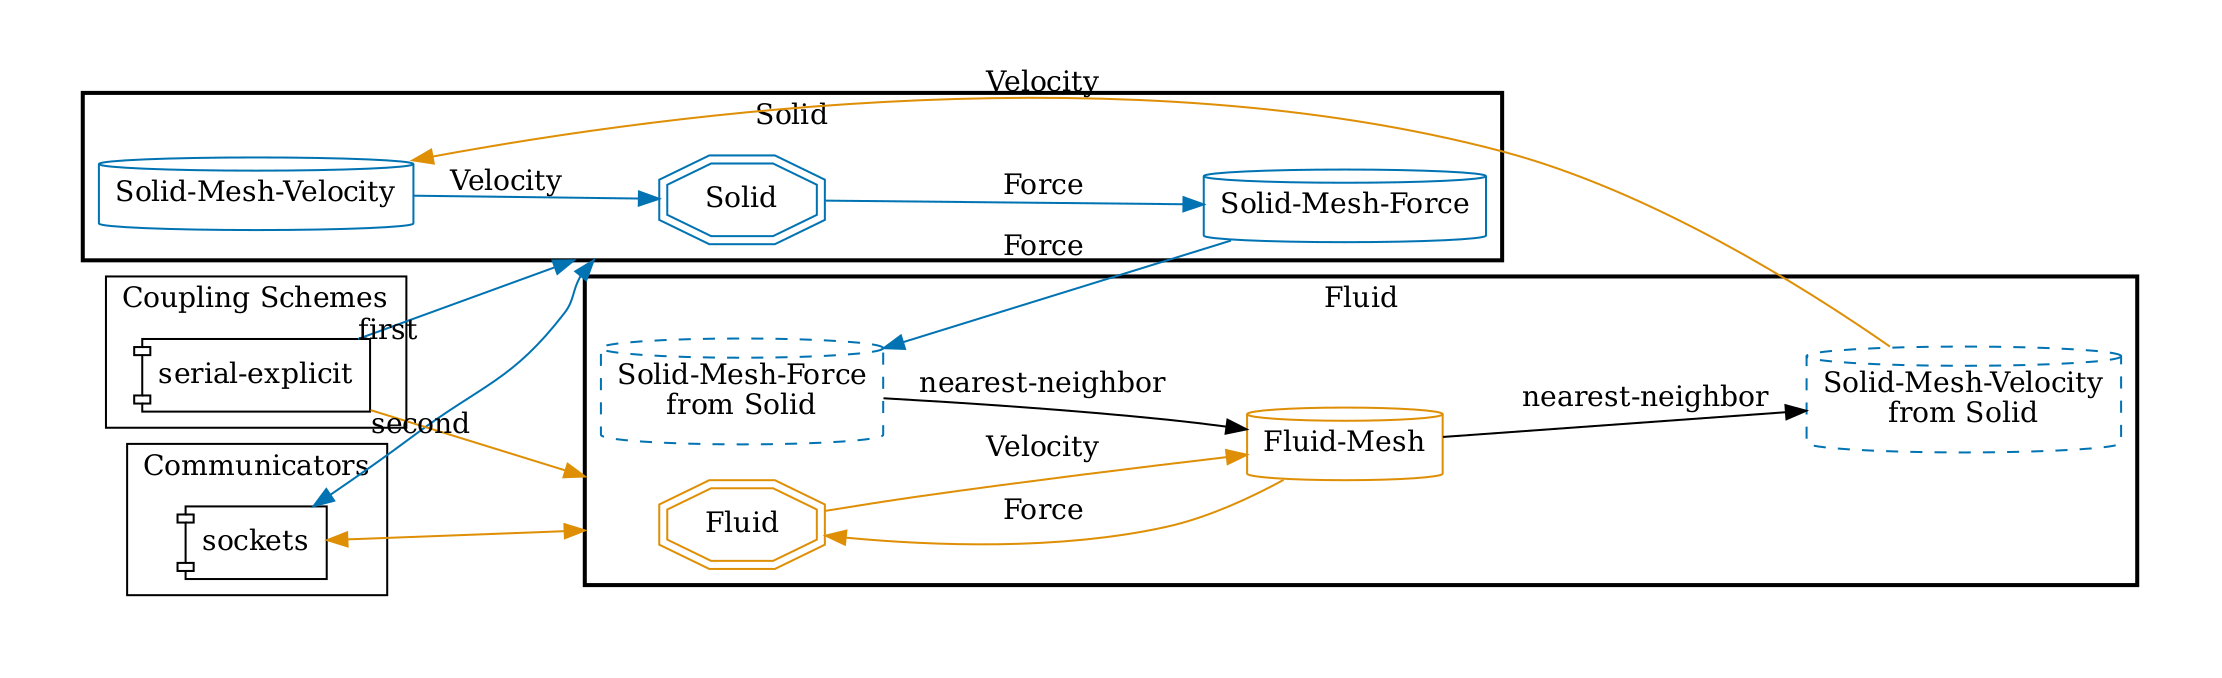
\includegraphics[width=0.9\textwidth]{images/openfast-dummy-coupling-scheme.png}
	\caption{Coupling scheme between OpenFAST, named Solid, and the dummy Fluid solver. The figure was created from the \textit{precice-config.xml} using the \textit{config visualizer tool}\protect\footnotemark.}
	\label{fig:openfast:coupling}
\end{figure*}

\footnotetext{\url{https://precice.org/tooling-config-visualization.html}}

\begin{comment}
Case dummy-turbine
\begin{itemize}
\item Explain the setup
\begin{itemize}
\item Couple OpenFAST to a dummy fluid solver
\item OpenFAST computes a NREL 5MW turbine with a fixed rotor to avoid problems due to the moving mesh
\item Fluid solver is implemented as dummy: No CFD calculation takes place
\item The dummy creates a mesh on which data from OpenFAST is read and writes back constant values
\item Allows to explore the mapping and data exchange
\item Can be used for regression tests in the future (use in challenges)
\end{itemize}
\item Explain the mesh use of OpenFAST
\begin{itemize}
\item OpenFAST has two internal meshes of the turbine surface with different vertices
\item Force mesh: Used to store and compute the surface force
\item Velocity mesh: Used to store and compute the flow velocity
\item Possibility to let OpenFAST map between the two meshes
\item Both meshes can be accessed via the C++ API
\item We want to use preCICE for the mapping
\item A similar coupling setup is employed by \cite{Taschner:2022} who also uses both meshes
\item Maybe add a visualization of the coupling scheme to clarify the mesh use\\
\end{itemize}
\end{itemize}
\end{comment}



\subsection{Coupling OpenFAST with OpenFOAM}

The second example case implements the coupling of OpenFAST to the CFD tool OpenFOAM. It employs the same coupling scheme and mesh use as the previous case. However, the Fluid mesh is now more complex. The main obstacle for a successful coupling is 

Case cfd-turbine
\begin{itemize}
	\item Explain the setup
	\begin{itemize}
		\item Couple OpenFAST to OpenFOAM
		\item The coupling scheme and mesh use is identical to the dummy
		\item Now we are dealing with a different mesh on the fluid solver
		\item Main obstacle: The OpenFOAM adapter is not designed to implement a coupling with a solver using the actuator line method. How to map between the line mesh in OpenFAST (Figure )\ref{fig:mesh:fast} and the volume mesh in OpenFOAM (Figure \ref{fig:mesh:foam})?
	\end{itemize}
	\item Explain how the current setup works
	\begin{itemize}
		\item Define a cellSet inside the OpenFOAM domain (Figure \ref{fig:mesh:foam}) to which OpenFAST is coupled
		\item Write the rotor and tower data to this subdomain
		\item Read velocity data from this subdomain
		\item The mapping from line to volume and back is done by preCICE, but probably wrong
	\end{itemize}
	\item How should the turbine be represented in OpenFOAM?
	\begin{itemize}
		\item Volume mesh / cellSet
		\item Surface mesh / patch
		\item ALM implementation (eg with turbinesFoam)\\
	\end{itemize}
\end{itemize}

\newpage
\begin{figure*}[h]
	\centering
	\begin{subfigure}{0.7\textwidth}
		\centering
		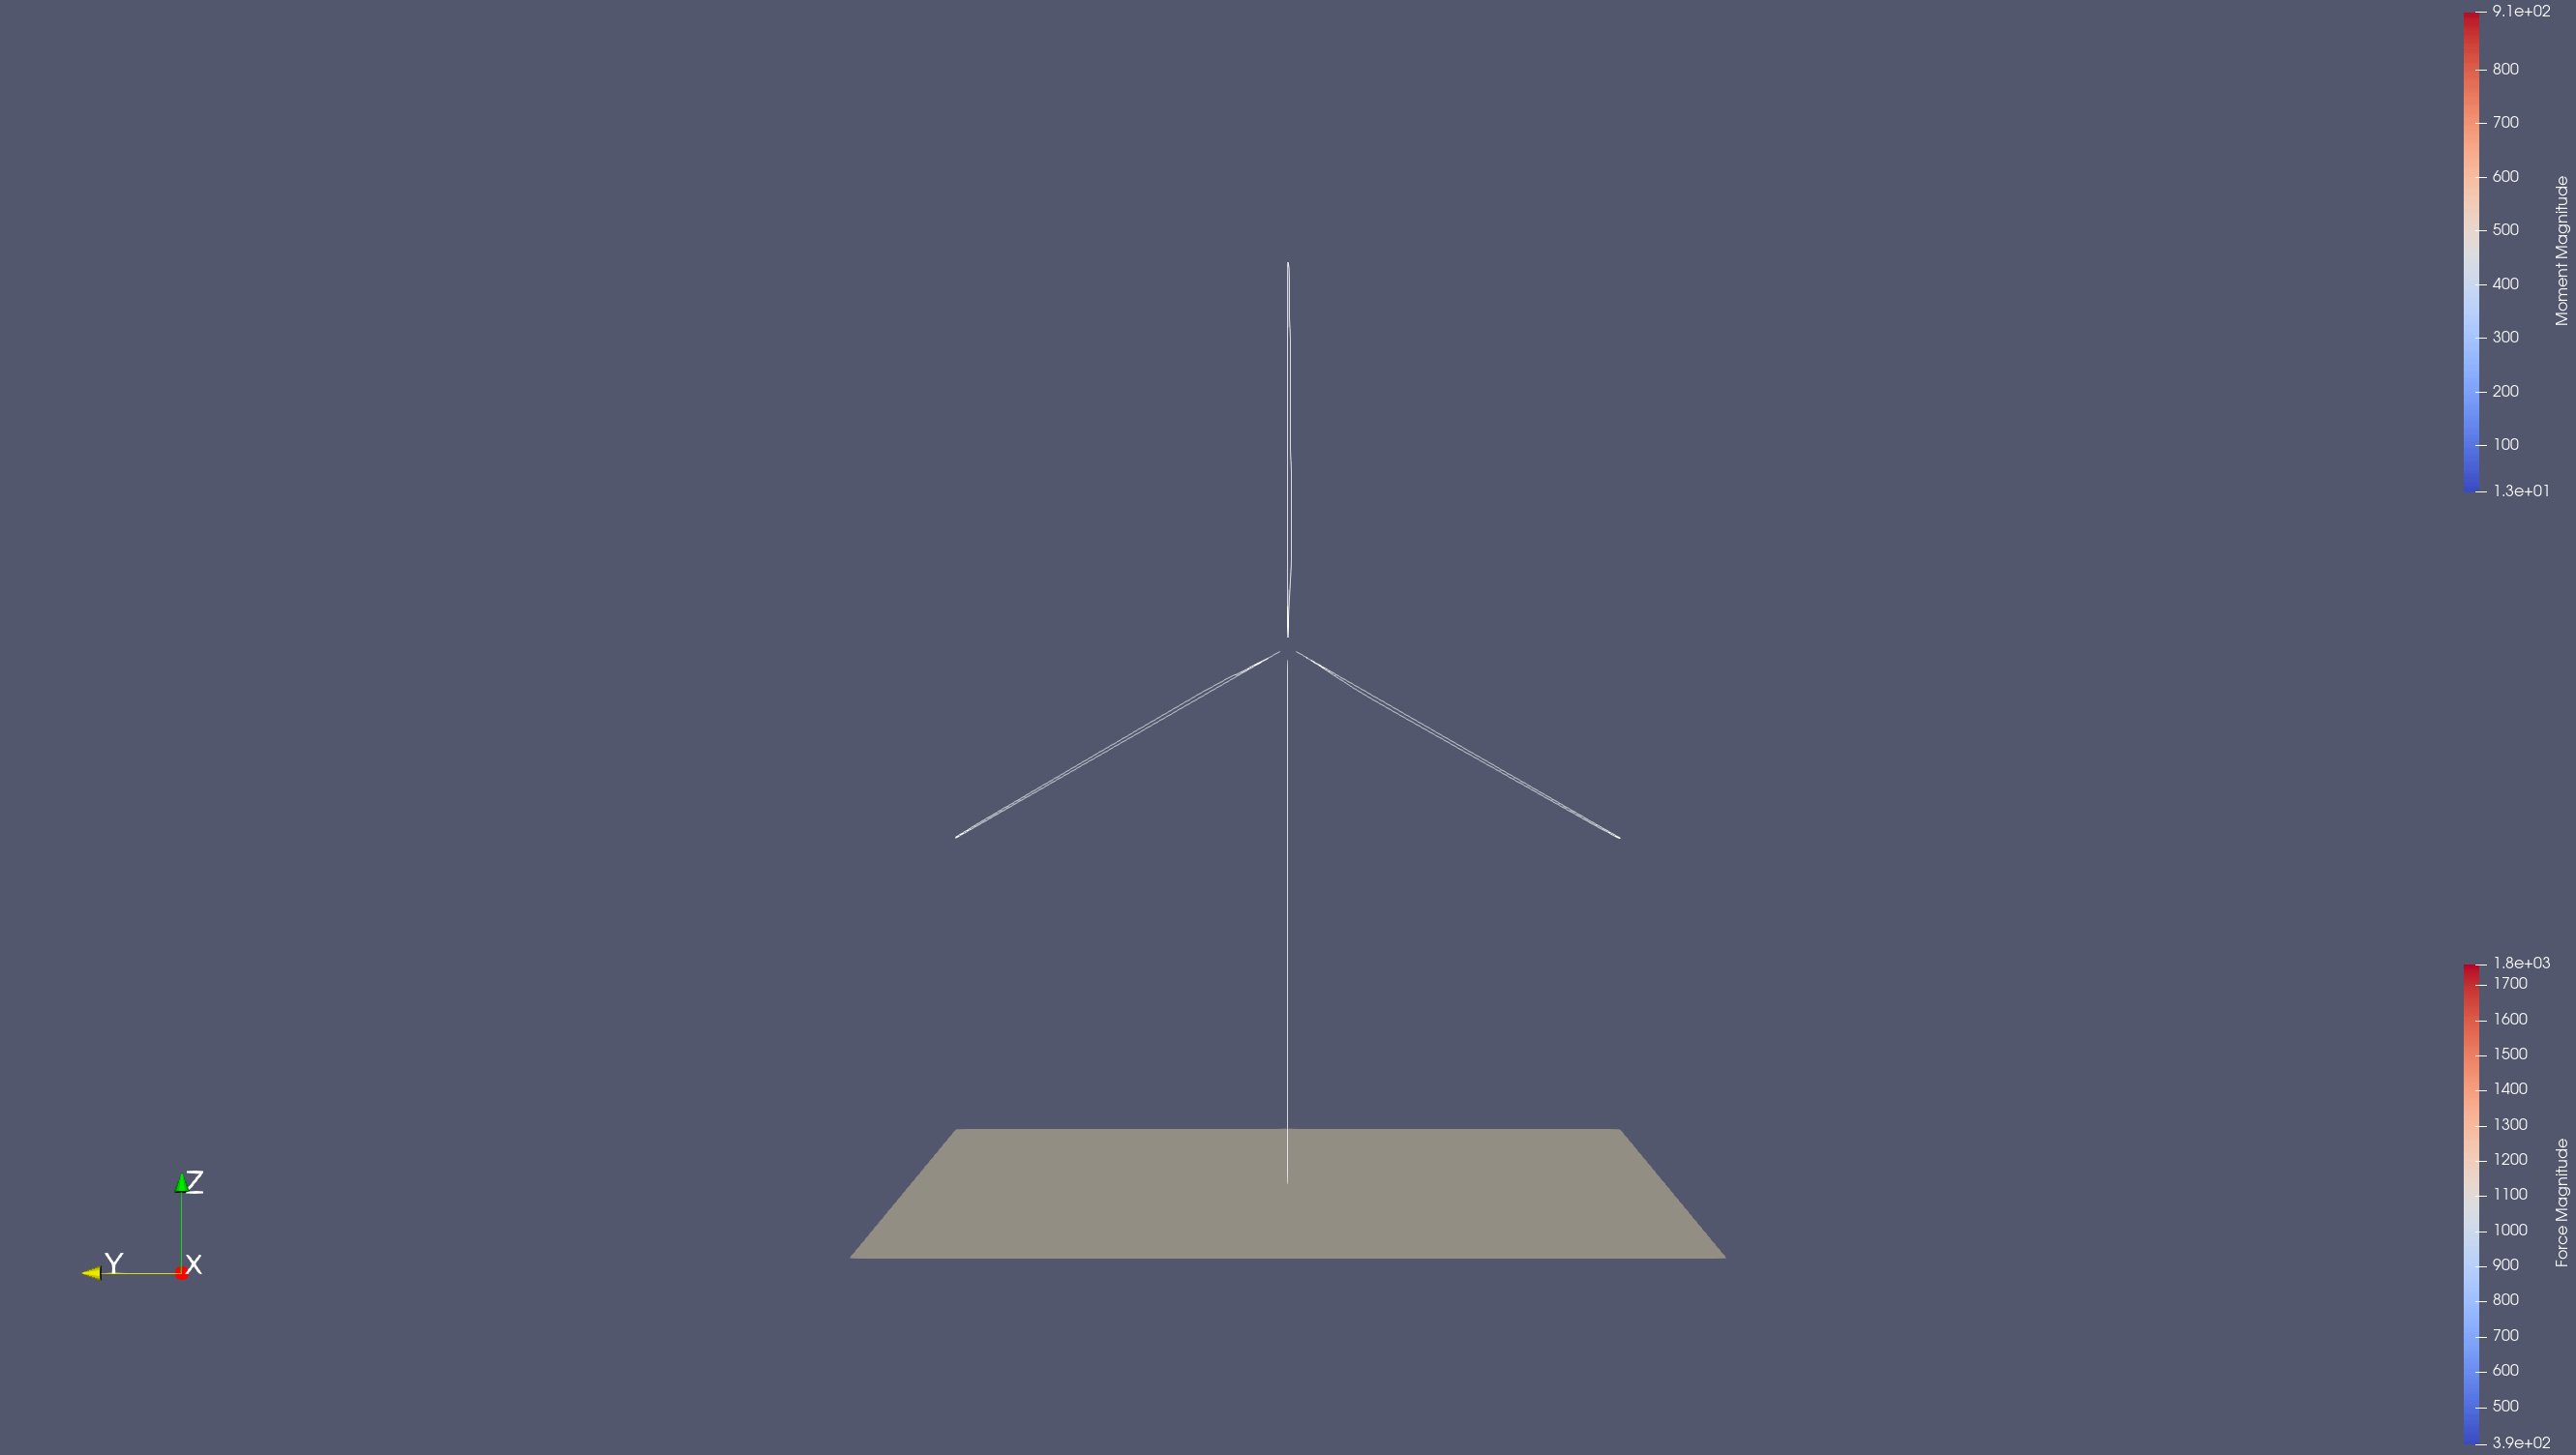
\includegraphics[width=\linewidth]{images/openfast-turbine-mesh.png}
		\caption{Line representation of the turbine in OpenFAST}
		\label{fig:mesh:fast}
	\end{subfigure}
	\vspace{2pt}
	\begin{subfigure}{0.7\textwidth}
		\centering
		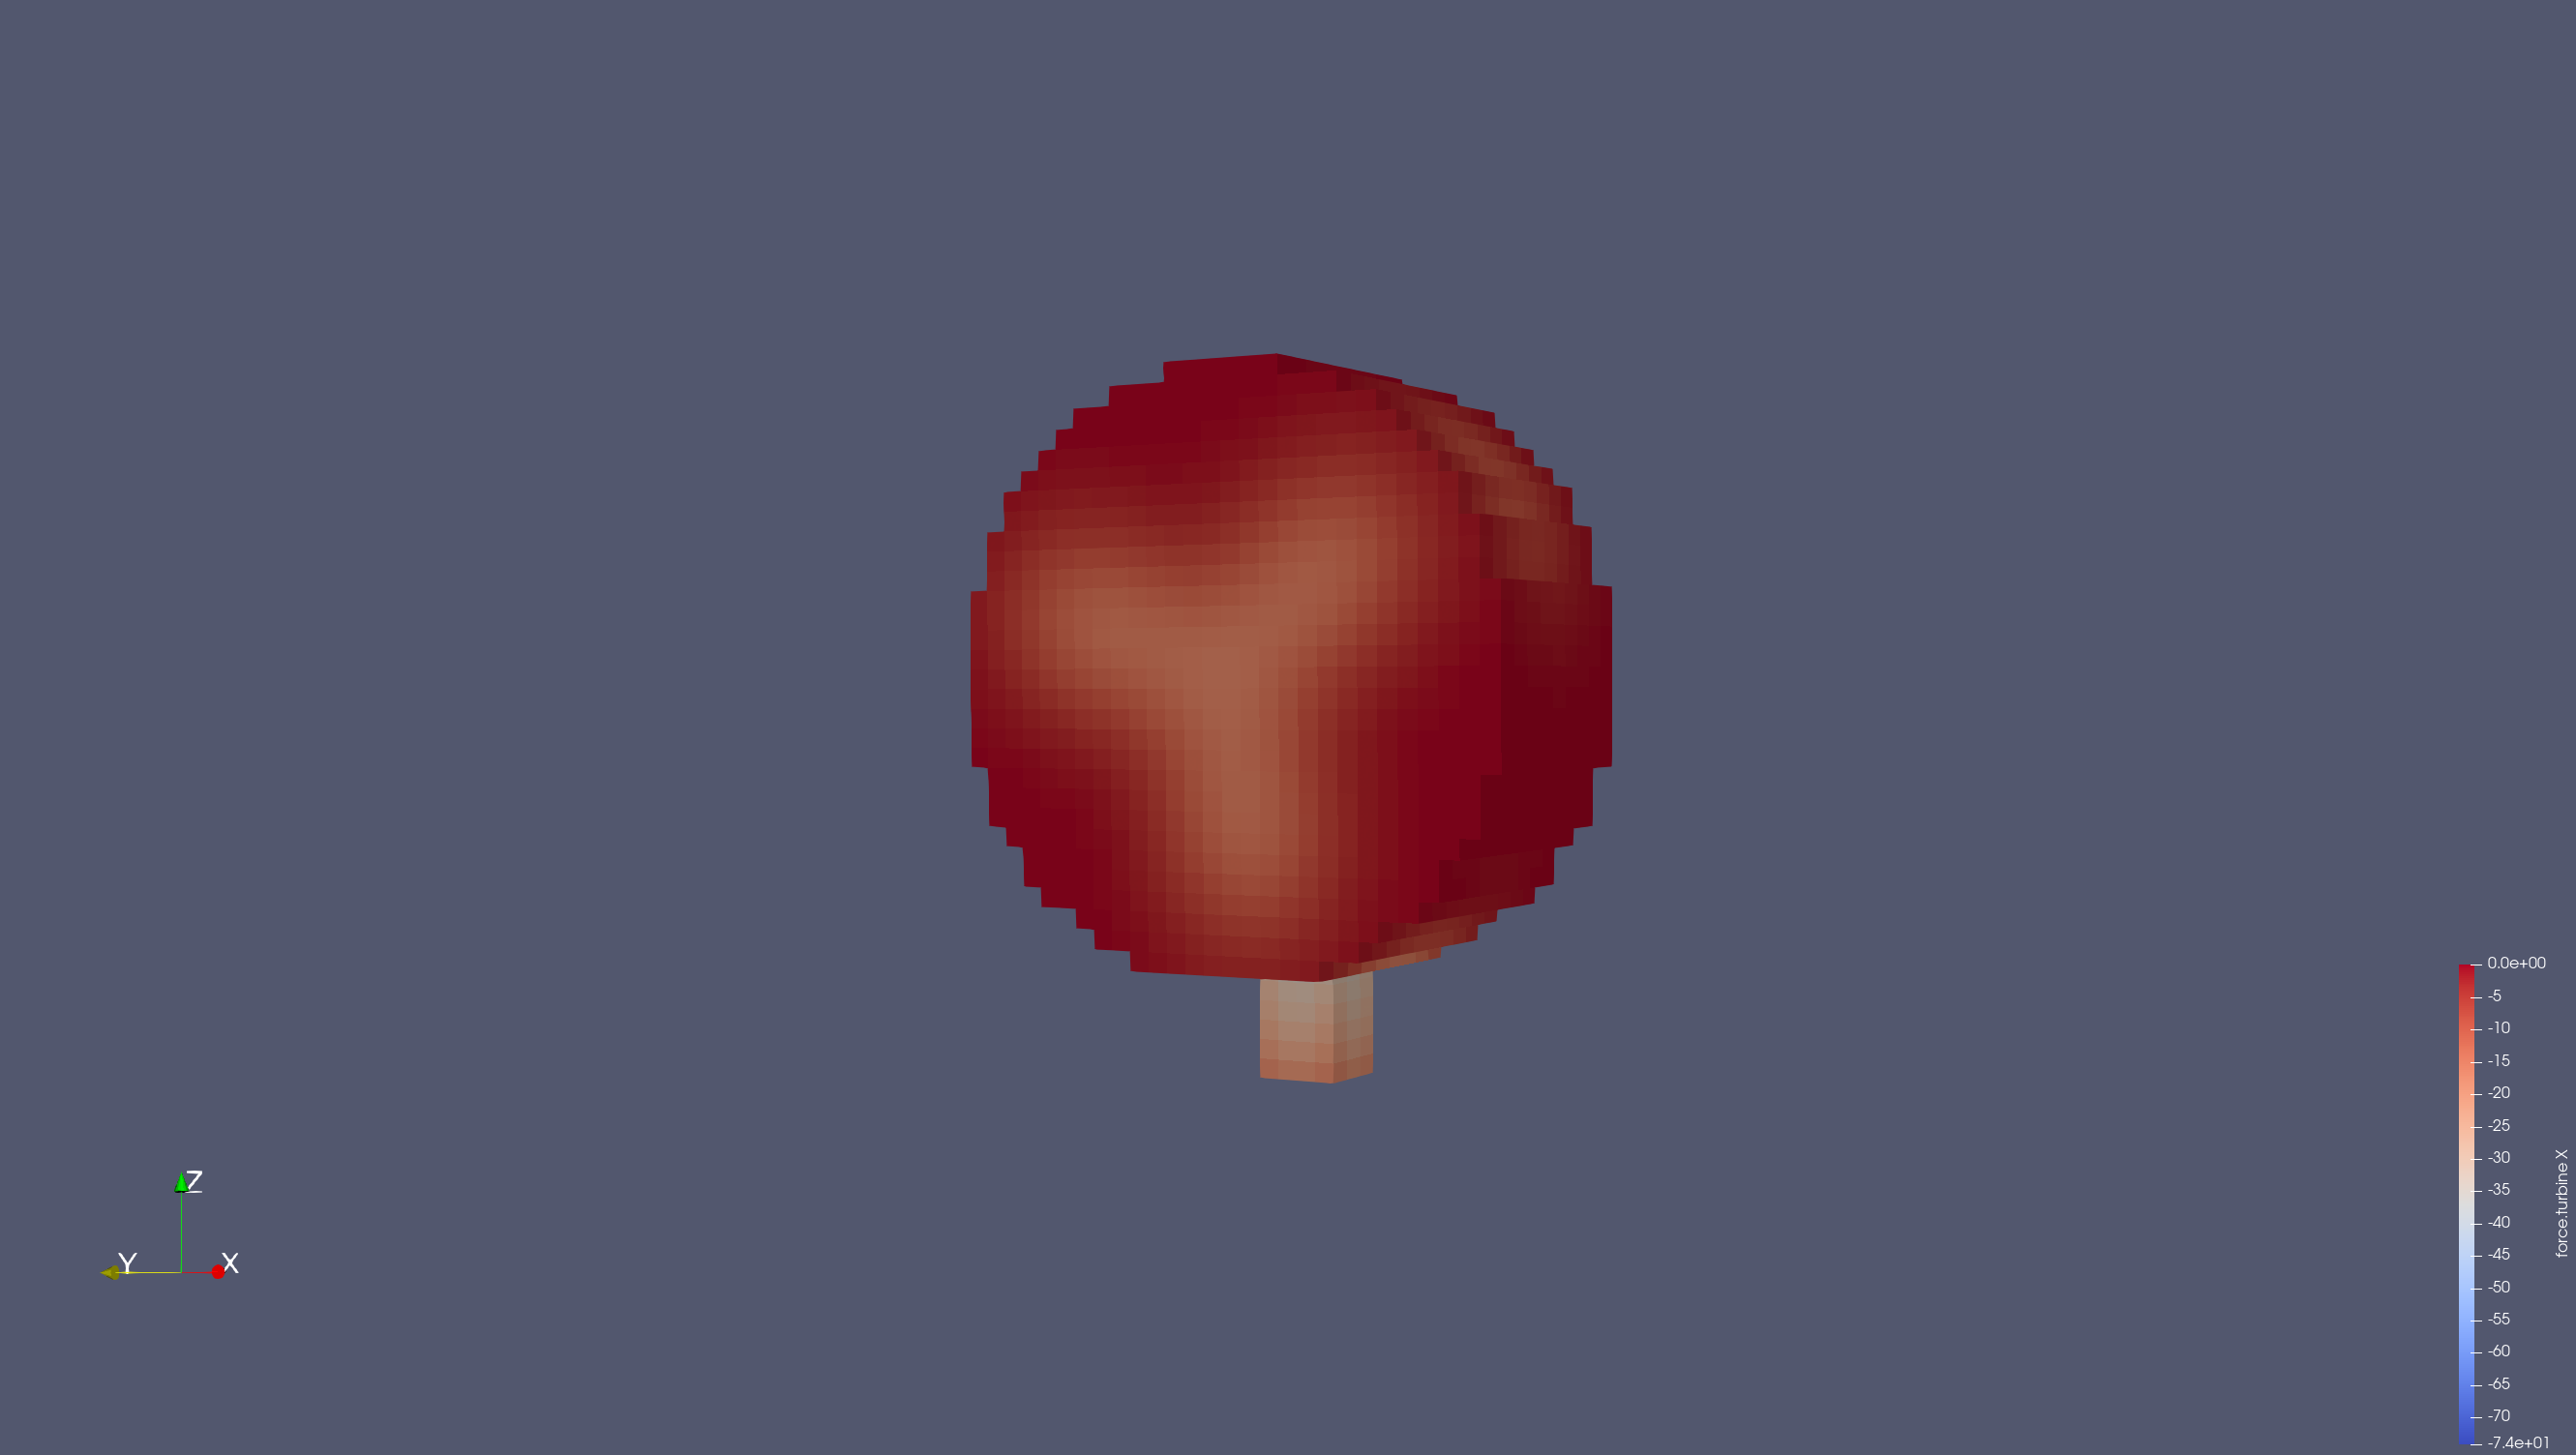
\includegraphics[width=\linewidth]{images/openfoam-turbine-mesh.png}
		\caption{Volume representation of the flow field immediately around the turbine in OpenFOAM}
		\label{fig:mesh:foam}
	\end{subfigure}
	\caption{Mesh differences between OpenFAST and the CFD solver OpenFOAM. OpenFAST uses the Actuator Line Model to represent blades and towers in the flow field, while OpenFOAM calculates the whole flow field.}
	\label{fig:mesh}
\end{figure*}



\section{Challenges}
\label{section:challenges}

What are the next steps in the coupling of OpenFAST via preCICE? This section aims to give an overview of the upcoming tasks to guide interested developers in their endeavour. 

\subsection{Mapping turbine data between actuator lines and volume meshes}

The most pressing issue is to implement a correct mapping. As seen in chapter \ref{section:cases}, the mapping depends not only on the preCICE-OpenFAST adapter, but also on the preCICE adapter of the CFD solver. In our case, we face problems because the OpenFOAM adapter was not designed for the implementation of ALM. In particular, the volume coupling functionalities are not sufficient. It is possible to retrieve velocity data from a volume. But it is not possible to write force or pressure gradient data on a volume. However, this functionality is needed to implement a bidirectional coupling for this FSI case. I see two solutions to this problem:\\
\textbf{Solution 1: Map in the OpenFAST adapter}\\
The code\footnote{\url{https://gitlab.com/whiffle-public/aspfast} (visited on 28.12.2023)} from AspFAST provides a possible solution. The tool to connect OpenFAST and GRASP is published under a MIT license and can therefore be re-used without limitations. It implements useful mapping functions in the main script \textit{aspast.cpp}. To communicate from OpenFAST to the CFD solver, the functions \textit{calcBodyForce}, \textit{uniformBodyForce} and \textit{diskBodyForce} are used. To understand the mapping from CFD to OpenFAST, look into the functions \textit{sampleVelocity} and \textit{calcVelocity}. Including similar functions in the OpenFAST adapter could help to address mapping problems. It is still unclear how the mapped force values would then be transferred to a volume mesh in OpenFOAM.\\[12pt]
\textbf{Solution 2: Modify the OpenFOAM adapter}\\
Another solution is to add the missing functionality in the OpenFOAM adapter. For the coupling setup, the Fluid-Fluid (FF) module of the adapter is used. For a correct coupling, OpenFOAM needs to include the updated field values of force or pressure gradient from OpenFAST. But the OpenFOAM adapter only supports the exchange of pressure as field value. To change this, we need to adapt the class \textit{PressureGradient.C} of the FF module. A code section to write pressure gradient data on a cellset should be added. Have a look in the class \textit{Pressure.C} of the FF module to get an idea how to access and write field values in OpenFOAM in general.

Inside OpenFOAM, the pressure gradient is stored as the boundary condition of the velocity field U. Therefore, we need to import the velocity field U in the class \textit{PressureGradient.C} and use appropriate commands from OpenFOAM to set its boundary condition. Setting the boundary condition on a cellset and not on a wall or inlet might be tricky.

As an additional remark, the OpenFOAM library turbinesFoam\footnote{\url{https://github.com/turbinesFoam/turbinesFoam} (visited 14.12.2023)} \cite{Bachant:2018} might be useful. It implements the actuator line method with different solvers like pimpleFoam. The solvers are modified to perform the ALM computation. It is not clear yet how this could be of use, as we want to perform the ALM computation of the turbine in OpenFAST and map the results to OpenFOAM, not do the whole computation in OpenFOAM.

\begin{comment}

\begin{itemize}
	\item Problem: The OpenFOAM adapter is not designed for the implementation of ALM
	\item We need to get velocity from a volume section --> possible
	\item We need to set force or pressure gradient on a volume section --> not possible
	\item Solution 1: Do the mapping in the OpenFAST adapter
	\begin{itemize}
		\item Something very similar has been done by AspFAST (LINK)
		\item The MIT license of the software allows to re-use it without limitations
		\item What exactly needs to be done?
		\begin{itemize}
			\item Look into aspfast.cpp
			\item Understand how the mapping from OpenFAST to the CFD solver is done in the functions \textit{calcBodyForce}, \textit{uniformBodyForce} and \textit{diskBodyForce}
			\item Understand how the mapping from the CFD solver to OpenFAST works in the functions \textit{sampleVelocity} and \textit{calcVelocity}
		\end{itemize}
		\item Includes smearing of the actuator data which is good
		\item Possible Problem: I add volume data to the mesh in the OpenFAST adapter that the OpenFOAM adapter is not able to write to FOAM afterwards --> think about
	\end{itemize}
	\item Solution 2: Modify the OpenFOAM adapter
		\begin{itemize}
			\item Adapt the PressureGradient.C class of the FF module
			\item Include code to write pressure gradient on a cellset
			\item Take structure from Pressure.C class
			\item Problem: How to write the pressure gradient on a field in OpenFOAM?
			\item Pressure gradient seems to be the boundary condition of the velocity field U --> this is settable
			\item Requires the correct import of the velocity field and the correct retrieval of its boundary field --> give the commands you know
			\item Not sure if you can also set the pressure gradient on the pressure field itself but dont think so
			\item Open: How to do smearing if necessary\\
		\end{itemize}
	\item Additional remark: The OpenFOAM library turbinesFoam\footnote{\url{https://github.com/turbinesFoam/turbinesFoam} (visited 14.12.2023)} \cite{Bachant:2018} might be useful. It implements the actuator line method with different solvers like pimpleFoam in OpenFOAM. The solvers are modified to perform the ALM computation. It is not clear yet how this could be of use, as we want to perform the ALM computation of the turbine to OpenFAST and map the results to OpenFOAM, not do the whole computation in OpenFOAM.
\end{itemize}
\end{comment}

\subsection{Improve code maturity}

To railguard the further development, a regression test should be implemented. The dummy fluid solver from chapter \ref{section:cases:dummy} can be used as a simple coupling participant to check calculations. The preCICE-FMI runner\footnote{\url{https://github.com/precice/fmi-runner/tree/main} (visited on 06.01.2024)} may serve as an example on how to write the test, place it in the GitHub repository and execute it automatically with GitHub workflows.

Once a mature coupling to OpenFOAM is achieved, the coupling should be verified. Previous work \cite{Taschner:2022} provides a benchmark case to cross-verify the coupling of a single NREL 5MW turbine with five other research LES codes.
\begin{comment}
\begin{itemize}
	\item Write a regression test (using the dummy fluid solver)
	\item Create a first test case with documentation
	\item Verify simulation results against simulations done with AspFAST and other tools (\cite{Taschner:2022} gives some benchmark cases)\\
\end{itemize}
\end{comment}

\subsection{Enable coupling with multiple turbines}

A future version of the adapter may include the coupling of multiple turbines in OpenFAST with one OpenFOAM instance. The OpenFAST C++ API allows to run multiple instances of OpenFAST to simulate wind park scenarios with FAST.FARM. But how do you communicate the results of multiple turbines to preCICE, and how do you organize the coupling to the CFD solver? This scenario increases the complexity in both adapters involved in the coupling setup. Again, a look into the AspFAST code could provide insight into how to deal with those challenges.

A different option may be the use of the preCICE Micro manager\footnote{\url{https://precice.org/tooling-micro-manager-overview.html} (visited on 06.01.2024)}. It is a tool to manage many micro simulations and couple them to one macro simulation. However, it must be said that the manager was not designed with large-scale FSI simulations in mind.
\begin{comment}
\begin{itemize}
	\item OpenFAST C++ API allows to run multiple instances of OpenFAST for wind park scenarios
	\item How do you connect them to preCICE? 
	\item How do you define the different coupling scenarios?
	\item Possibly use the MacroMicro manager of preCICE to deal with the coupling of multiple domains\\
\end{itemize}
\end{comment}


\subsection{Explore coupling scenarios with other CFD solver}

The current work is focused on the coupling of OpenFAST with OpenFOAM for the simple fact that it is the only suitable CFD solver in the preCICE ecosystem. The coupling of other tools like GRASP, NaluWind or YALES2 via preCICE might be interesting to create a simulation environment where CFD solvers could be swapped easily. Simulation results could be compared mor readily and the individual strengths of each program leveraged depending on the simulation case. However, this setup comes with the additional effort of developing preCICE adapters for the other CFD programs. As the tools above are already coupled to OpenFAST with mature, verified tools, this should only be done if it adds real benefit to the research community.

\begin{comment}
\begin{itemize}
\item Are there currently other CFD solvers coupled to preCICE that would be interesting?
\item Otherwise interesting candidates are: YALES2, GRASP, NaluWind
\item Most of them have native coupling tools for OpenFAST already\\
\end{itemize}

Additional remarks
\begin{itemize}
	\item The OpenFOAM library turbinesFoam\footnote{\url{https://github.com/turbinesFoam/turbinesFoam} (visited 14.12.2023)} \cite{Bachant:2018} might be useful. It implements the actuator line method with different solvers like pimpleFoam in OpenFOAM. The solvers are modified to perform the ALM computation. It is not clear yet how this could be of use, as we want to perform the ALM computation of the turbine to OpenFAST and map the results to OpenFOAM, not do the whole computation in OpenFOAM.
\end{itemize}
\end{comment}


\section{Conclusion}
\label{section:conclusion}

\begin{itemize}
	\item First coupling of OpenFAST and preCICE was presented
	\item Coupling with a dummy solver and OpenFOAM was discussed
	\item Although a proof of concept was achieved, some challenging tasks remain to enable a full coupling to CFD solvers
	\item How to map between OpenFAST and an arbitrary CFD solver? Where to place the mapping and smearing algorithm for the ALM method?
	\item This work may serve as a starting point
	\item Has the potential to be developed into a viable open-source alternative for the coupling of OpenFAST to different CFD solvers
\end{itemize}


\section*{Acknowledgments}

I am grateful to Prof. Axelle Viré who accepted me as a visiting researcher and made this work possible. Many thanks to her and Evert Ewald for the discussions and hints during our meetings. Extended thanks to Benjamin Uekermann, who enabled my visit at TU Delft in the first place and provided feedback along the way. Lastly, I want to thank the wonderful crowd of PhD researchers in the wind energy department who made my time in Delft memorable.

%% Bibliography

\printbibliography

%% Appendix
\begin{comment}
\section*{Appendix}

Possible points to include in the Appendix
\begin{itemize}
\item Files from the OpenFOAM adapter with hints on how to modify them
\item Files from AspFAST with hints on how to reuse the code for our mapping
\end{itemize}
\end{comment}


\end{document}
